\chapter{イントロダクション}
\label{ch:intro}
\ref{ch:intro}章では我々が行う研究の背景について述べる。
まず\ref{sec:intro_background}節では地球大気でのオゾンの重要性と高エネルギー粒子の降り込みとオゾンの減少について述べる。
次に\ref{sec:intro_privious}節では、先行研究で明らかになったことと、問題点について述べる。
最後に\ref{sec:intro_porpose}節では\ref{sec:intro_privious}節の内容を踏まえて本研究の目的について述べていく。


\section{研究背景}
\label{sec:intro_background}
% \begin{itemize}
%     \item 高エネルギー粒子のモデル結果と観測結果の差を示す
%     \item EPPからO3の現象までの流れを示す
% \end{itemize}
% ここでNOの略称を紹介し、以後NOと略す
地球大気の大部分は窒素分子\ce{N2}と酸素分子\ce{O2}で占められているが、大気微量成分と呼ばれる\ce{N2}と\ce{O2}以外の大気分子も地球環境に影響を与えている。
オゾン分子\ce{O3}もその大気微量成分の1つであり、\ce{O3}の変動によって大気の放射バランスが変わり、地上の気候や気象に影響を与える可能性が指摘されている~\cite{rozanov2012influence,seppala2009geomagnetic}。
これまで、冷媒などに用いられたフロンガスなど人為的な原因によるオゾンの変動に着目した研究は行われてきた。
しかし、自然現象による原因の中でも、とくに太陽活動に伴う高エネルギー粒子の降り込み(EPP: Energetic Particle Precipitation)の影響によるオゾンの変動に関してシミュレーション結果と観測結果には大きな開きがあるため、十分な観測的理解には達していない(図\ref{fig:rozanov2012_seppala2009})。
\begin{figure}[htbp]
    \centering
    \begin{minipage}{\linewidth}
        \centering
        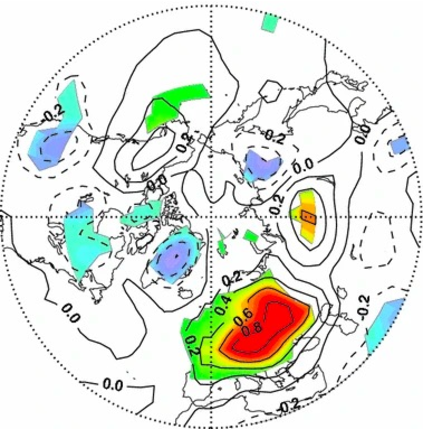
\includegraphics[scale=0.6]{master_thesis_contents/master_thesis_fig/rozanov2012_fig12.pdf}
        \subcaption{シミュレーション結果(最大で$0.8\, \mathrm{K}$の増加、~\cite{rozanov2012influence}より引用)}
        \label{fig:rozanov2012_fig12}
    \end{minipage}
    \begin{minipage}{\linewidth}
        \centering
        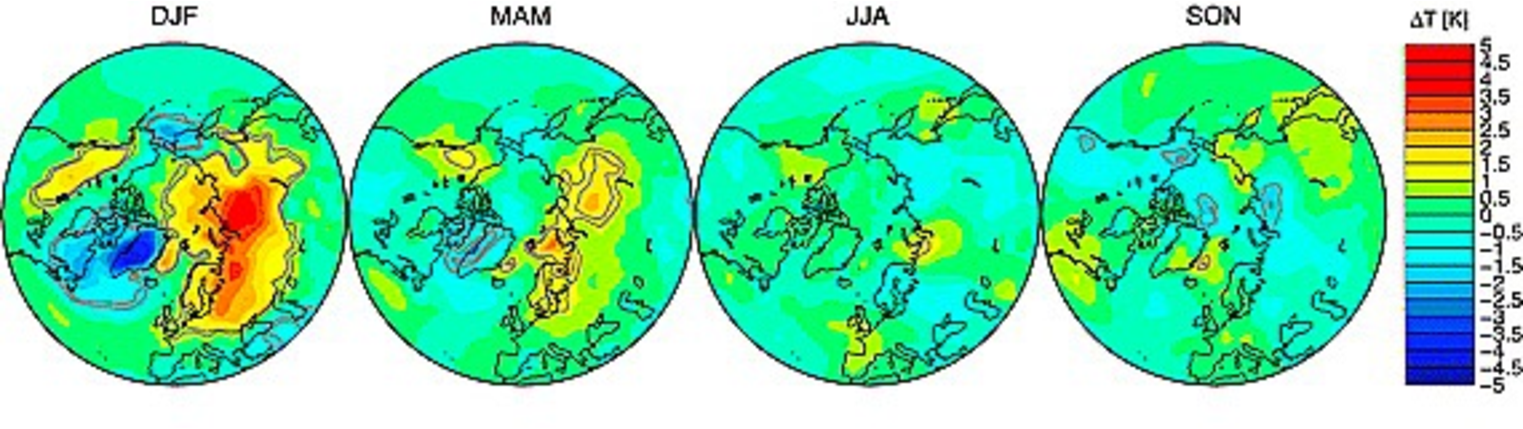
\includegraphics[scale=0.6]{master_thesis_contents/master_thesis_fig/seppala2009_fig3.pdf}
        \subcaption{観測データに基づいた統計結果(最大で$5\, \mathrm{K}$の増加、~\cite{seppala2009geomagnetic}より引用)}
        \label{fig:seppala2009_fig3}
    \end{minipage}
    \caption{EPP時の地表温度の変化$\Delta T\, \mathrm{[K]}$}
    \label{fig:rozanov2012_seppala2009}
\end{figure}
そこで我々の研究グループでは、EPPの影響によるオゾンの変動を観測的に明らかにすることを研究目的の1つとして研究を行っている。
EPPの影響によってオゾンの変動に影響を与えるまでには、図\ref{fig:epp_to_ozone_flow}のような流れで起きる。
\begin{figure}[htbp]
    \centering
    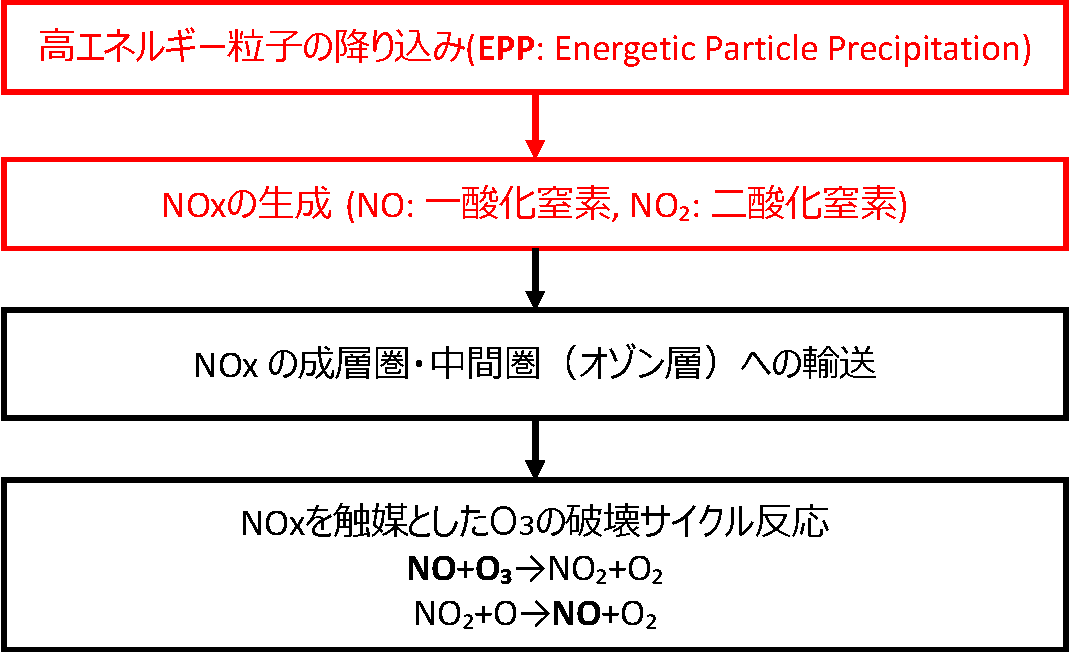
\includegraphics[width=\linewidth]{master_thesis_contents/master_thesis_fig/epp_to_ozone_flow.pdf}
    \caption{EPPからオゾン破壊までのフロー}
    \label{fig:epp_to_ozone_flow}
\end{figure}
まずEPPがあると、それによって\ce{NOx}と呼ばれる一酸化窒素\ce{NO}や二酸化窒素\ce{NO2}が生成される。
それが大気の輸送によって成層圏・中間圏に輸送されることにより、これらの反応式で表されるように\ce{O3}の破壊サイクル反応を起こす。


\section{先行研究の結果と課題}
\label{sec:intro_privious}
% \begin{itemize}
%     \item 衛星観測で示されたNOとO3の変動
%     \item ミリ波観測で示されたNOの短期変動と季節変動
%     \item 衛星観測では同じ場所での連続的な現象の観測が難しいこと
%     \item 衛星観測では、緯度方向にでしか議論が行われていないこと
%     \item ミリ波では夏に短期変動の観測ができないことを示す(観測手法でのトロムソの話につながる)
% \end{itemize}
先行研究では高エネルギー粒子の降込みによって\ce{NOx}が増加し、それがオゾンの変動に影響を与えていることが衛星観測のデータにて時間分解能が1日ではあるが示されている(図\ref{fig:lopez2005observation_fig3})~\cite{lopez2005observation}。
2003年10月28日にEPPがあったが、それと前後して\ce{NOx}の増加が確認されており、\ce{NOx}の増加があった地域に\ce{O3}の減少が確認されている。
\begin{figure}[htbp]
    \centering
    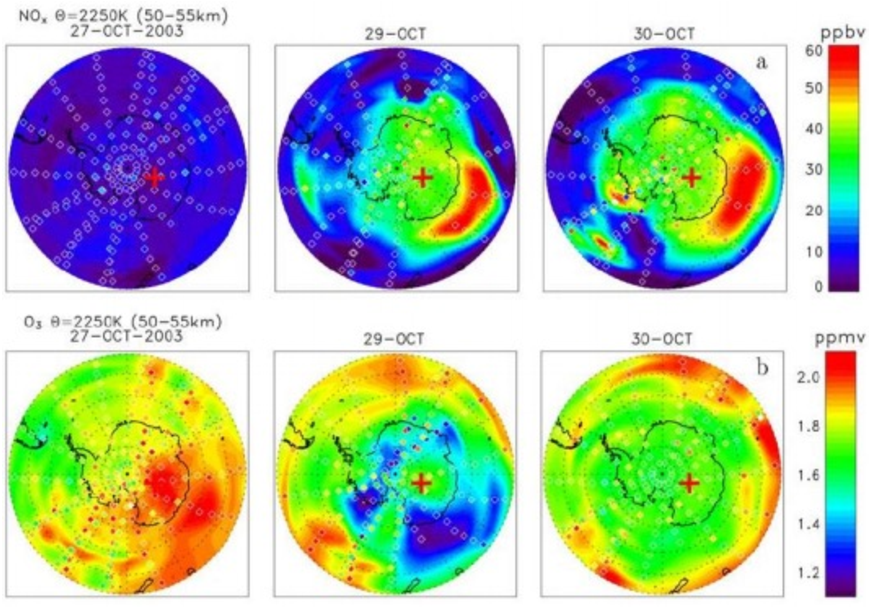
\includegraphics[width=\linewidth]{master_thesis_contents/master_thesis_fig/lopez2005observation_fig3.pdf}
    \caption{EPPイベントの前後での\ce{NOx}と\ce{O3}の変動(~\cite{lopez2005observation}より引用)}
    \label{fig:lopez2005observation_fig3}
\end{figure}
このように衛星観測では全球的な観測を行うことが可能ではあるが、時間分解能は比較的悪く、定点で連続的な現象の観測が難しいという課題がある。
その課題を克服するため、我々の研究グループではミリ波分光計(観測手法の詳細は\ref{ch:mm_obs}章)を用いた観測を行っている。


次に我々の研究グループで行われたミリ波分光計を用いた先行研究について話していく。
我々のグループでは2011年から南極昭和基地でミリ波分光による地上観測を行っている。
図\ref{fig:isono2014ground_fig5a}は2012年から2013年までの観測による解析結果である。
横軸が時系列になっていて月ごとに目盛りがふってあり、横軸において、黒色のエラーバーは\ce{NO}の存在量(厳密には柱密度。詳細は\ref{sec:derive_columndensity}節)を表している。
紫色の影の部分に関しては、それぞれの日で太陽が当たっていない時間を表している。
この結果より、季節にともなう長期的変動、冬には高エネルギー粒子によるものと考えられる短期変動が確認できた。
しかし、夏は太陽光による光解離の影響もあり高エネルギー粒子による影響と切り分けをすることができなかった。
\begin{figure}[htbp]
    \centering
    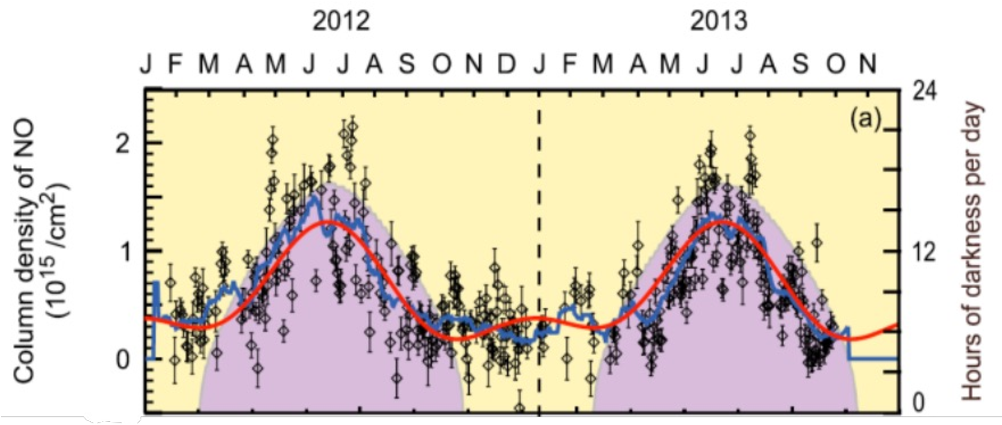
\includegraphics[width=\linewidth]{master_thesis_contents/master_thesis_fig/isono2014ground_fig5a.pdf}
    \caption{ミリ波分光計を用いた観測による南極・昭和基地での\ce{NO}の変動(~\cite{isono2014ground}より引用)}
    \label{fig:isono2014ground_fig5a}
\end{figure}
以上のことを踏まえて衛星観測とミリ波分光での地上観測による先行研究で明らかになったことと課題点についてまとめる。
\clearpage
\begin{itemize}
    \item 明らかになった点
    \begin{itemize}
        \item ミリ波分光を用いた地上観測(南極・昭和基地)
        \begin{itemize}
            \item 季節にともなう\ce{NO}の長期的変動
            \item EPPに伴う\ce{NO}の増加
        \end{itemize}
        \item 衛星観測
        \begin{itemize}
            \item EPPに伴う\ce{NO}の増加
            \item \ce{NO}の増加した地域にて見られた\ce{O3}の減少
        \end{itemize}
    \end{itemize}
    \item 課題点
    \begin{itemize}
        \item ミリ波分光を用いた地上観測(南極・昭和基地)
        \begin{itemize}
            \item 夏の\ce{NO}の短期変動の確認が難しい
        \end{itemize}
        \item 衛星観測
        \begin{itemize}
            \item 定点での連続的な観測が難しい
        \end{itemize}
    \end{itemize}
\end{itemize}
\ref{sec:intro_porpose}節では、これらの課題点を踏まえた本研究の目的について述べていく。


\section{本研究の目的と内容}
\label{sec:intro_porpose}
% \begin{itemize}
%     \item EPPからO3の現象までの流れの中でどこまでを扱うかを示す
% \end{itemize}
本研究では図\ref{fig:epp_to_ozone_flow}で示したフローの中でも上2つの関係について注目した(図\ref{fig:flow_and_porpose}中の赤枠)。
EPPについて、Dst指数と呼ばれる地磁気擾乱の大きさを表す指数と衛星観測による電子フラックスデータ、\ce{NOx}についてはミリ波観測による\ce{NO}スペクトルデータから導出した柱密度(柱密度の導出までの手法の詳細は\ref{ch:mm_analysis}章)をもとにして、お互いの関係性について調べることを研究目的としている。
\begin{figure}[htbp]
    \centering
    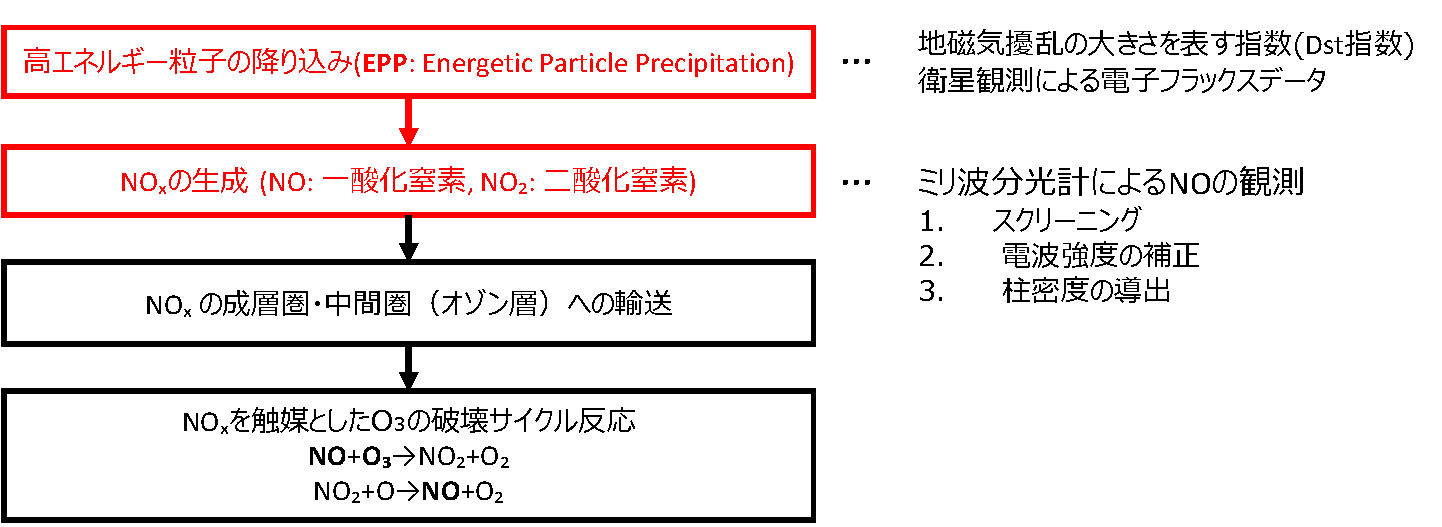
\includegraphics[width=\linewidth]{master_thesis_contents/master_thesis_fig/flow_and_porpose.pdf}
    \caption{図\ref{fig:epp_to_ozone_flow}と本研究の目的との対応}
    \label{fig:flow_and_porpose}
\end{figure}
